\documentclass[final,t]{beamer}
\usepackage{cmbright}
\usepackage[T1]{fontenc}
\usepackage{lipsum}  

%\usefonttheme[onlymath]{serif} %for math mode in serif

% poster template
\usepackage[orientation=portrait,scale=1.4,size=a0,debug]{beamerposter}
\setlength{\paperwidth}{48in} %size
\setlength{\paperheight}{36in}
\usetheme{zurichposter}

\definecolor{UMNgold}{RGB}{255,204,51}
\definecolor{UMNmaroon}{RGB}{122,0,25}

% references
\usepackage[bibstyle=authoryear, citestyle=authoryear-comp,%
hyperref=auto]{biblatex}
\bibliography{references}

% document properties
\title{\huge Some overcomplicated name}
\institute{\Large Further things you want to list}
\author{\Large Name and contact info}


%------------------------------------------------------------------------------
\begin{document}

\begin{frame}{}
\begin{columns}[t]

\begin{column}{.02\paperwidth} %spacing to left side of column 1 aka "padding"
\end{column}


%-----------------------------------------------------------------------------
%                                                                     COLUMN 1
% ----------------------------------------------------------------------------



\begin{column}{.225\paperwidth} %4 cols use .3, use .025 for the padding columns
	
	%"block"s are maroon and "alertblock"s are gold
	\begin{block}{Show me what you got}
		\small
		\begin{itemize}
			\item[\textcolor{UMNmaroon}{\textbullet}] something
			\item[\textcolor{UMNmaroon}{\textbullet}] something else
		\end{itemize}
	\end{block}
	
	\vskip2ex
	
    \begin{center}
       	
\includegraphics[width=\linewidth]{umn-logo.png}
    \end{center}
    \FloatBarrier %latex does weird shit so I use these
\end{column}

\begin{column}{.02\paperwidth} 	%shitty padding column
\end{column}

%-----------------------------------------------------------------------------
%                                                                     COLUMN 2
% ----------------------------------------------------------------------------

\begin{column}{.225\paperwidth}
	
	\begin{block}{something else}
		\small
		\lipsum[1]
		\vskip 1ex
		
		\begin{equation}
			\mathbold{B}(P_0) = \nonumber \frac{\mu_0}{4\pi}\int_{\partial \Omega} \frac{I d\mathbold{\ell}\times\mathbold{r}}{|\mathbold{r}|^3}
		\end{equation}
	\end{block}
	\vskip2ex
\end{column}

\begin{column}{.02\paperwidth}
\end{column} 
%-----------------------------------------------------------------------------
%                                                                     COLUMN 3
% ----------------------------------------------------------------------------

\begin{column}{.225\paperwidth}
	\begin{block}{The Tragedy of Darth Plagueis The Wise}
		\small 
		Darth Plagueis was a Dark Lord of the Sith so powerful and so wise, he could use the Force to influence the midi-chlorians to create life. He had such a knowledge of the dark side, he could even keep the ones he cared about from dying.
		\begin{figure}[h!]
			\begin{center}
				\hskip-5ex
				\resizebox{1\linewidth}{!}{% XCircuit output "class-e-op.tex" for LaTeX input from class-e-op.ps
\def\putbox#1#2#3#4{\makebox[0in][l]{\makebox[#1][l]{}\raisebox{\baselineskip}[0in][0in]{\raisebox{#2}[0in][0in]{\scalebox{#3}{#4}}}}}
\def\rightbox#1{\makebox[0in][r]{#1}}
\def\centbox#1{\makebox[0in]{#1}}
\def\topbox#1{\raisebox{-0.60\baselineskip}[0in][0in]{#1}}
\def\midbox#1{\raisebox{-0.20\baselineskip}[0in][0in]{#1}}
   \scalebox{0.5826}{
   \normalsize
   \parbox{9.08333in}{
   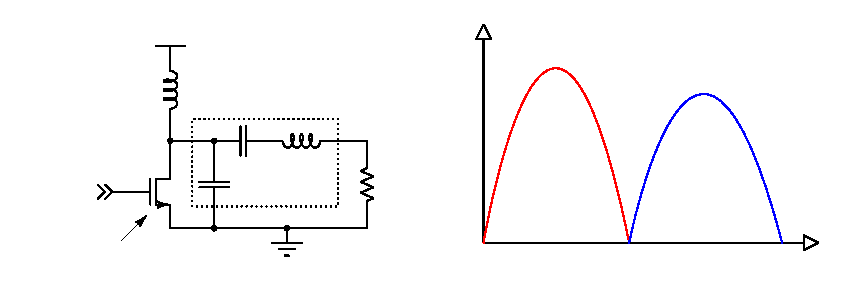
\includegraphics[scale=1.71644]{class-e-op}\\
   % translate x=345 y=905 scale 0.22
   \putbox{2.09in}{2.26in}{1.20}{Amplifier Output}%
   \putbox{2.43in}{2.01in}{1.20}{Network}%
   \putbox{1.01in}{2.09in}{1.20}{RFC}%
   \putbox{0.09in}{1.09in}{1.20}{Gate}%
   \putbox{0.09in}{0.84in}{1.20}{Drive}%
   \putbox{0.59in}{0.18in}{1.20}{Gate Drive}%
   \putbox{4.18in}{1.09in}{1.20}{Load}%
   \putbox{6.01in}{2.59in}{1.20}{Vds}%
   \putbox{7.68in}{2.34in}{1.20}{Id}%
   \putbox{6.76in}{0.09in}{1.20}{Time}%
   \putbox{1.59in}{2.84in}{1.20}{48V}%
   } % close 'parbox'
   } % close 'scalebox'
   \vspace{-\baselineskip} % this is not necessary, but looks better
} 
			\end{center}
		\end{figure}
	\end{block}

	\vskip2.5cm
	\begin{center}
		
\includegraphics[width=\linewidth]{umn-logo.png}
	\end{center}
	\FloatBarrier
	\vskip2ex
	
	\begin{exampleblock}{Kafka}
		\small 
		One morning, when Gregor Samsa woke from troubled dreams, he found himself transformed in his bed into a horrible vermin. He lay on his armour-like back, and if he lifted his head a little he could see his brown belly, slightly domed and divided by arches into stiff sections.
		
		The bedding was hardly able to cover it and seemed ready to slide off any moment. His many legs, pitifully thin compared with the size of the rest of him, waved about helplessly as he looked. "What's happened to me? " he thought. It wasn't a dream. His room, a proper human
	\end{exampleblock}
	
\end{column}

\begin{column}{.02\paperwidth}
\end{column}

%-----------------------------------------------------------------------------
%                                                                     COLUMN 4
% ----------------------------------------------------------------------------
\begin{column}{.225\paperwidth}

		\begin{block}{\LaTeX}	
		\small 
	The road to wisdom? — Well, it's plain\\
	and simple to express:\\ 
	Err\\ 
	and err\\ 
	and err again \\
	but less \\
	and less \\
	and less.
		\end{block}
		\vskip1ex
	
	\begin{alertblock}{Conclusions}	
		shit doesn't work
	\end{alertblock}


				
				
	\end{column}

\end{columns}

\end{frame}

\end{document}
